\section{Industrial design}

In this section, the industrial design will be explained and especially shown with pictures to have an idea of how the product will look. The design part was done by the ECAL student. The indutrial designer presented different solutions, they were then discussed together with the other member of the group. The solutions were also presented to the nurses and some old people to define which one is the more understandable and easy to use.

\subsection{Tablet}

The color of the shield is the orange. This color is hot and represent the positivity. It also is visible color and not agressive. The screen size is 7 inches with a resolution of 800x480. It is big enough to display readable messages and pictures.

The case has a certain thickness to allow users to have a better grip. The device can have 2 postures, one more vertical and one more horizontal. The user can then watch the tablet sitting down and holding in his hands or the device can be watched like a digital photo frame.

The design of the tablet is shown in the figure \ref{fig:vesta design}.

\begin{figure}[!htb]
    \centering
    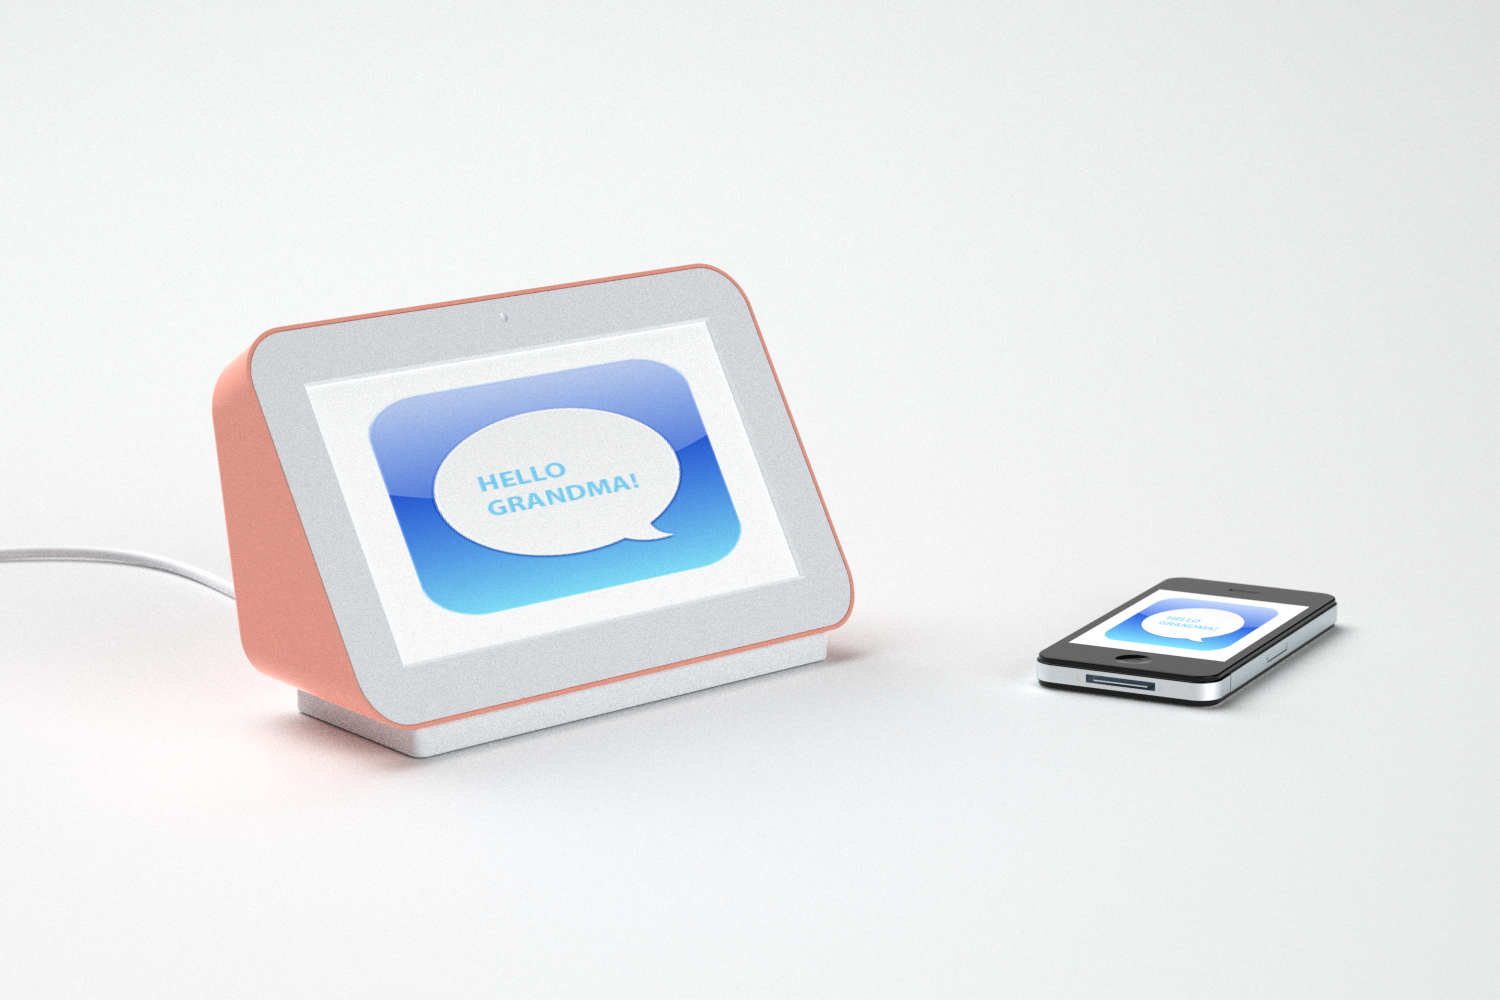
\includegraphics[width=0.7\textwidth,keepaspectratio]{chap/designFig/VestaRender4.png}
    \caption{Vesta tablet design}
    \label{fig:vesta design}
\end{figure}

On the left, the vesta tablet on the charging station. On the right, an iphone for scale.

\subsection{Charging station}

The charging station is wireless, it works with induction. More and more devices in the market allow to charge the battery wirelessly. To charge the tablet's battery, the tablet need to be located on the charging station. The advantage of this station is that the old people doesn't need to plug a small cable like micro USB into the tablet to charge it. The charging station method is much easier to use.

\begin{figure}[!htb]
    \centering
    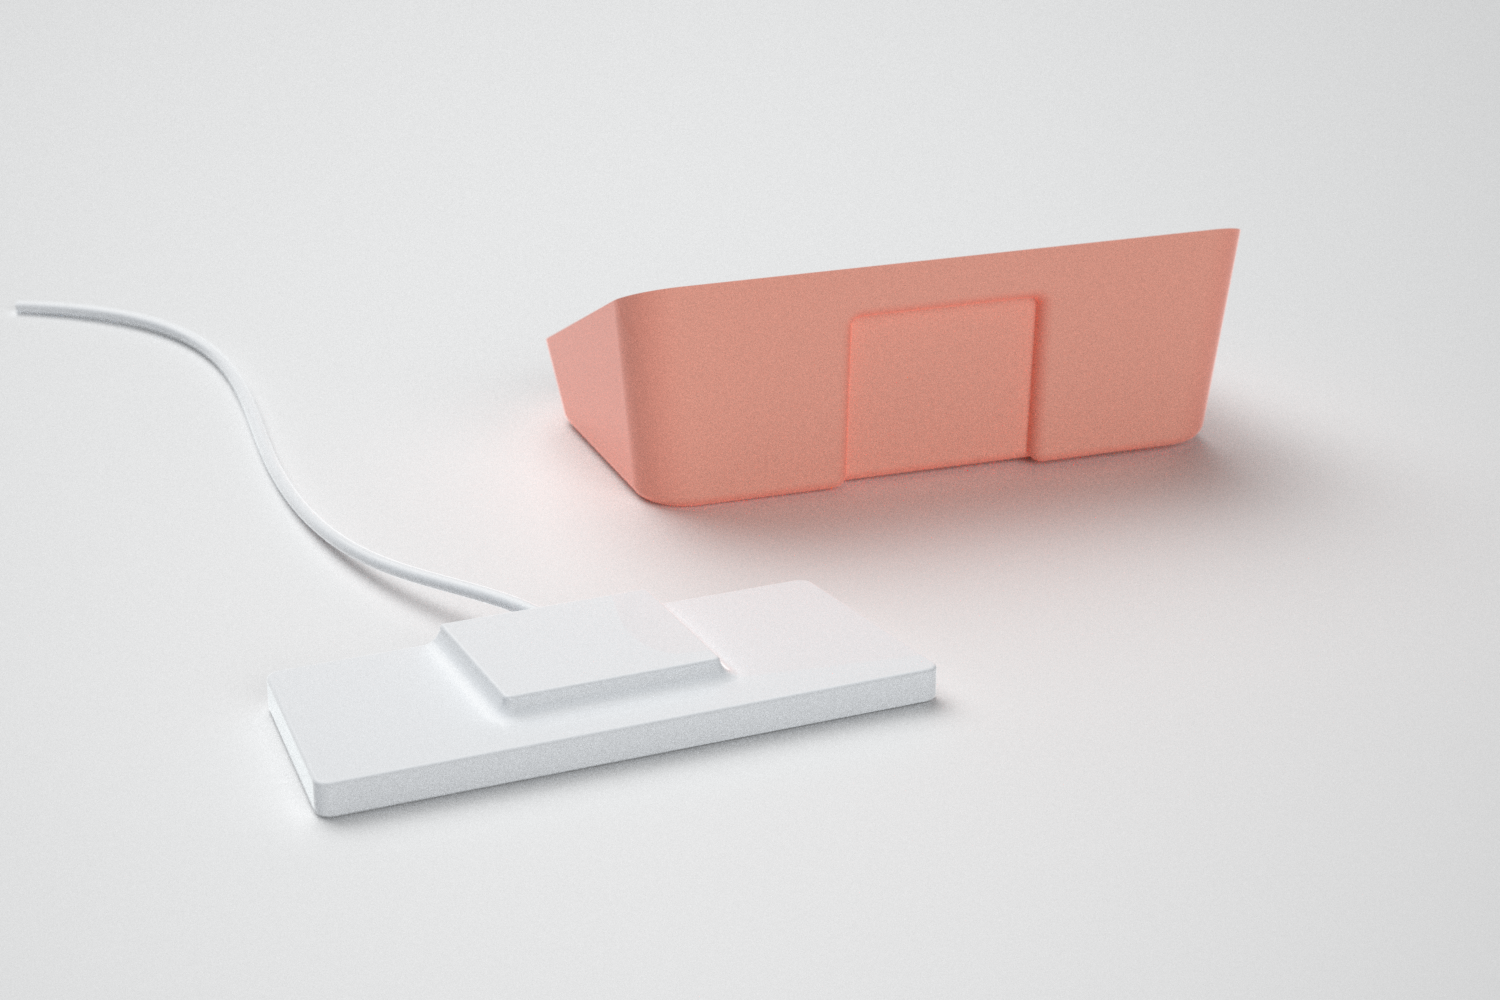
\includegraphics[width=0.7\textwidth,keepaspectratio]{chap/designFig/VisioRender7.png}
    \caption{Charging station}
    \label{fig:charging station}
\end{figure}

On the left, the inductive charging station. On the right, the vesta tablet in horizontal position.

\clearpage

\subsection{Software design}

The software located on the tablet need to be very easy to use and understandable by an old people. Different designs were imagined and compared.

The graphical interface of the software is shown in the figure \ref{fig:soft design}.

\begin{figure}[!htb]
    \centering
    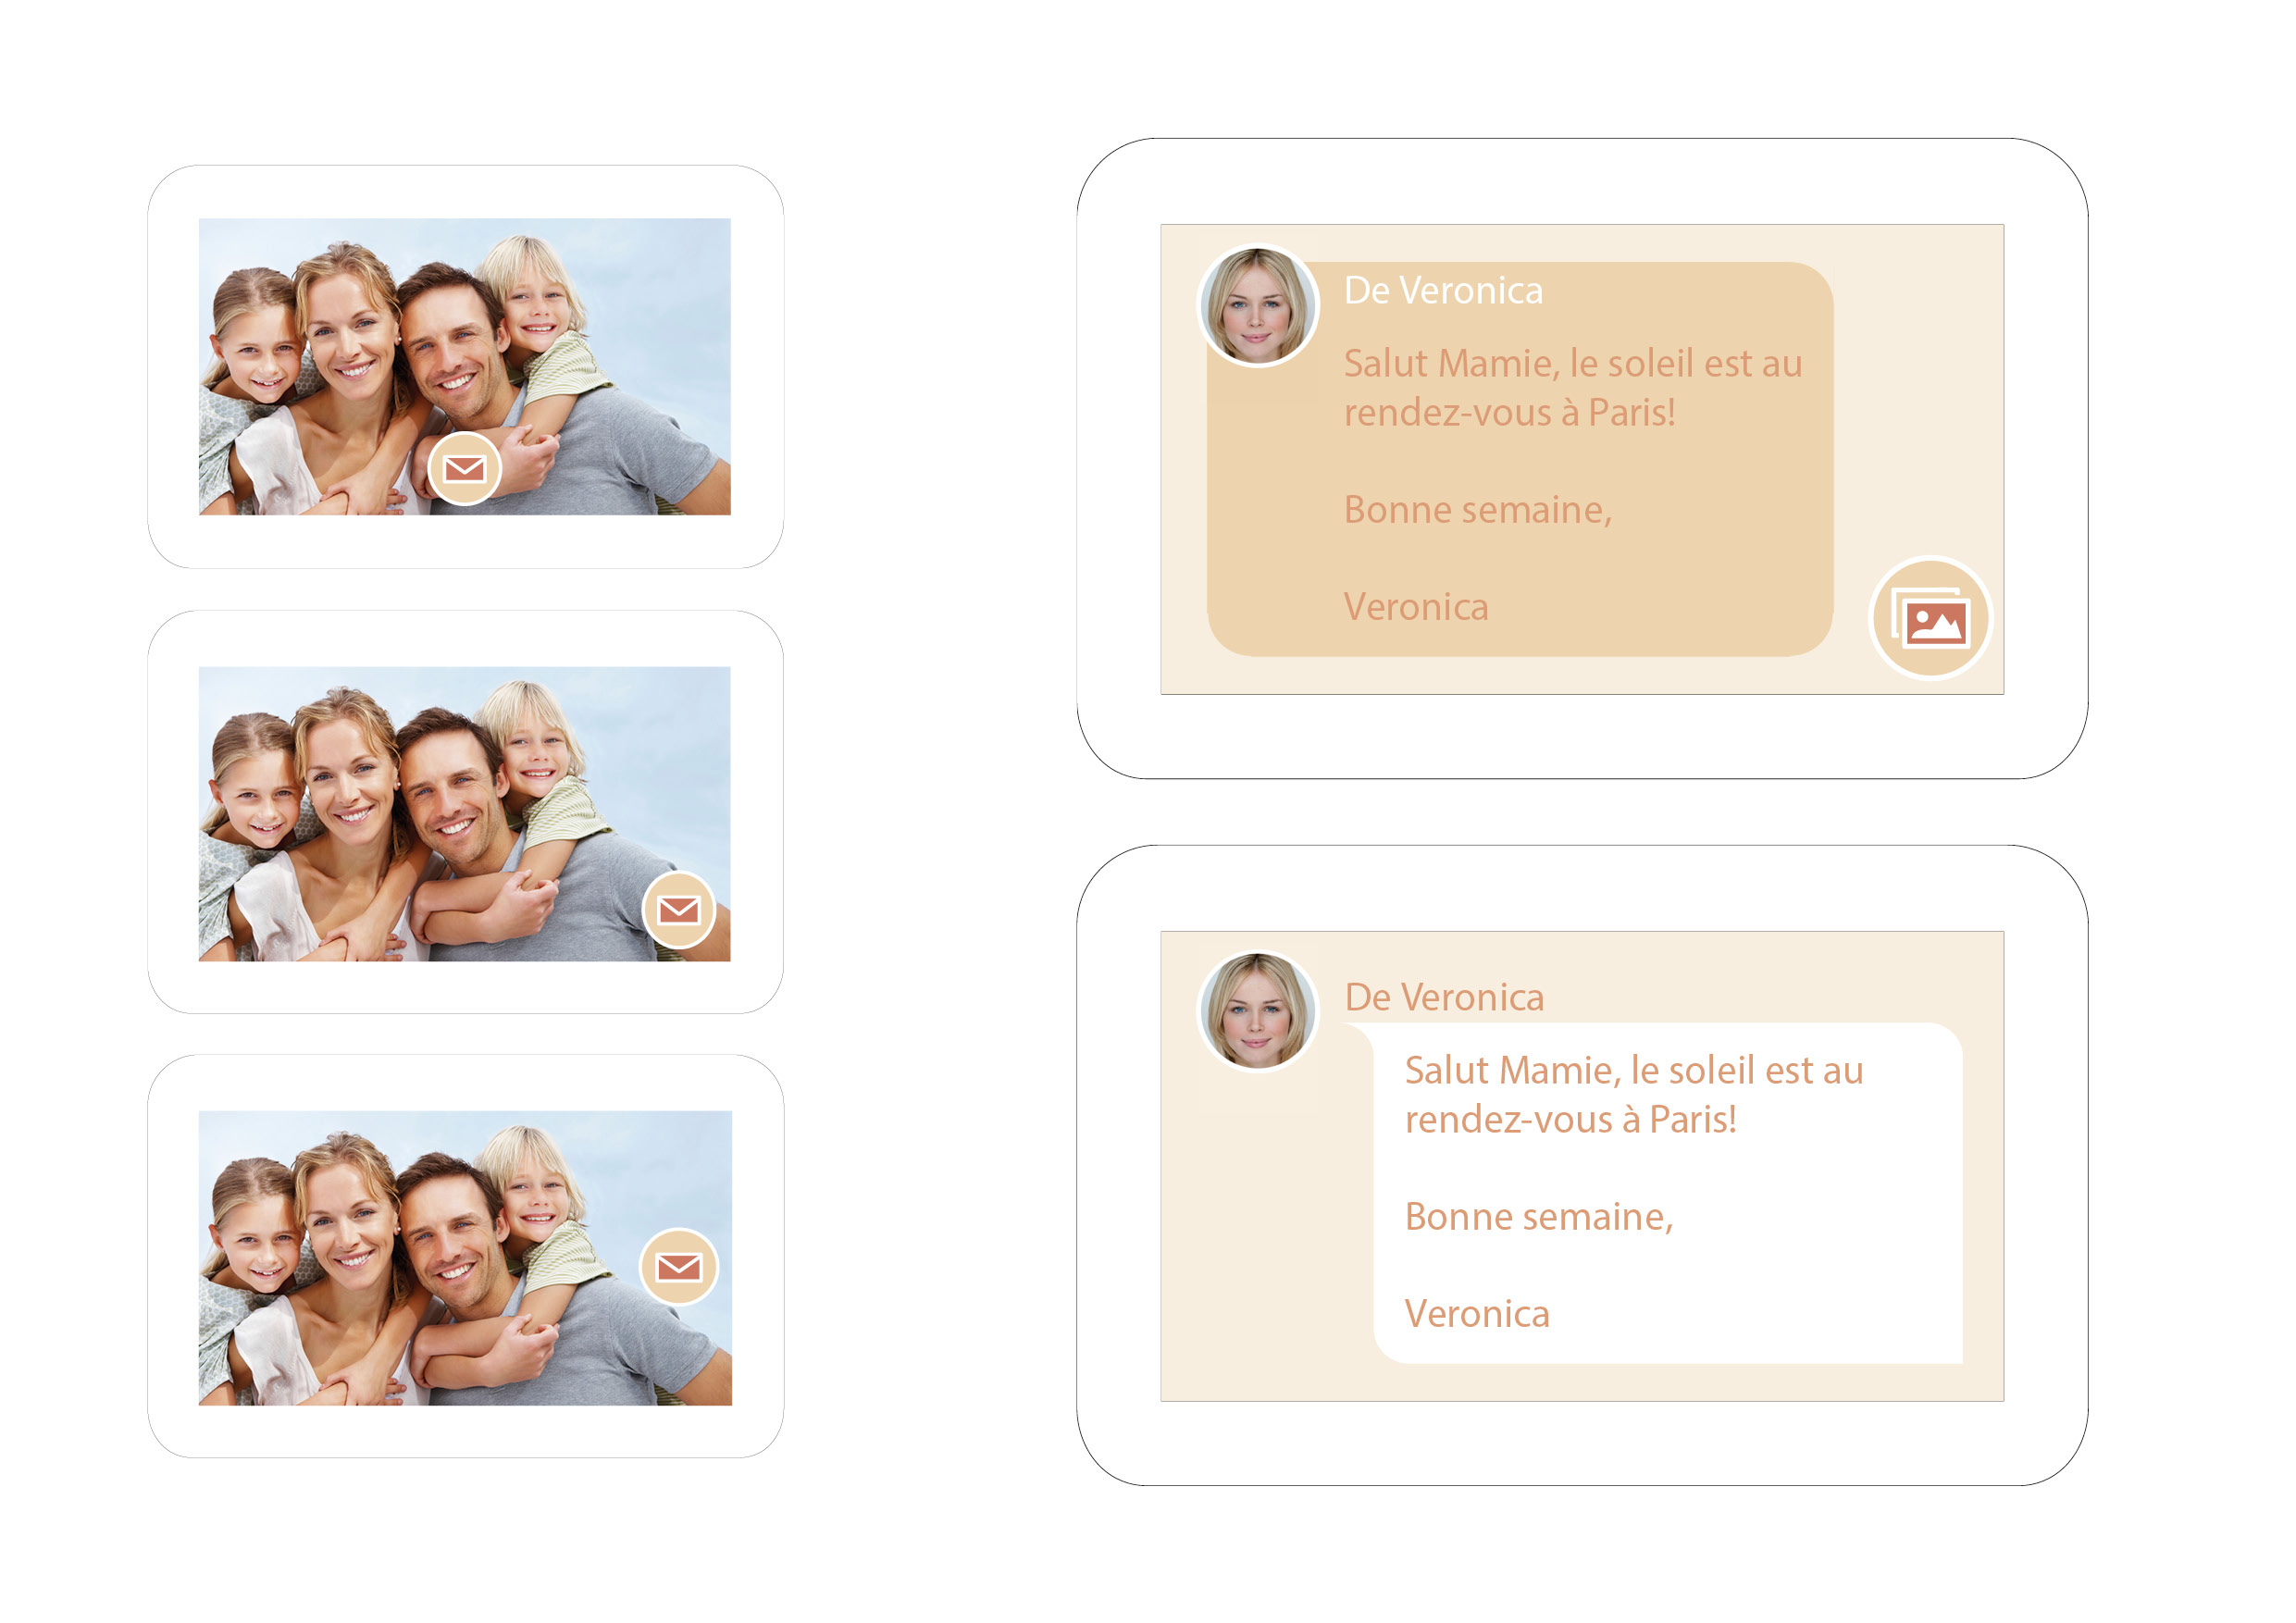
\includegraphics[width=0.9\textwidth,keepaspectratio]{chap/designFig/vesta_design.jpg}
    \caption{Software design}
    \label{fig:soft design}
\end{figure}

On the left the software design imagined for the picture display with the button to display the text message. And on the right, the design of the text message display with the picture of the sender and the button to return to the picture.
